In pursuit of scientific advancement across many domains, experiments are becoming exceedingly sophisticated in order to probe physical systems at increasingly smaller spatial resolutions and shorter timescales.  
These order of magnitude advancements have lead to explosions in both data volumes and richness leaving domain scientists to develop novel methods to handle growing data processing needs.  

Simultaneously, machine learning (ML), or the use of algorithms that can learn directly from data, is leading to rapid advancements across many scientific domains~\cite{Carleo:2019ptp}. 
Recent advancements have demonstrated that deep learning (DL) architectures based on structured deep neural networks are versatile and capable of solving a broad range of complex problems. 
The proliferation of large datasets like ImageNet~\cite{imagenet}, computing, and DL software have led to the exploration of many different DL approaches each with their own advantages. 

In this review paper, we will focus on the fusion of ML and experimental design to solve critical scientific problems by accelerating and improving data processing and real-time decision making. 
We will discuss the myriad of scientific problems that require fast ML, and we will outline unifying themes across these domains that can lead to general solutions. 
Furthermore, we will review the current technology needed to make ML algorithms run fast, and we will present critical technological problems that, if solved, could lead to major scientific advancements. 
An important requirement for such advancements in science is the need for openness.  
It is vital for experts from domains that do not often interact to come together to develop transferable solutions and work together to develop open-source solutions.  

Much of the advancements within ML over the past few years has originated from the use of heterogeneous computing hardware. 
In particular, the use of graphics processing units (GPUs) has enabled the development of large DL algorithms~\cite{gpus1,gpus2,gpus3}.  
The ability to train large artificial intelligence (AI) algorithms on large datasets has enabled algorithms that are capable of performing sophisticated tasks. 
In parallel with these developments, new types of DL algorithms have emerged that aim to reduce the number of operations so as to enable fast and efficient AI algorithms. 

\begin{tcolorbox}
%Can we define here: What is Fast (which is somewhat vague)?  Here we mean accelerated and/or real-time beyond traditional computing paradigms. 
Within this review paper, we refer to the concept of \textit{\textbf{Fast Machine Learning in Science}} as the integration of ML into the experimental data processing infrastructure to enable and accelerate scientific discovery. Fusing powerful ML techniques with experimental design decreases the ``time to science" and can range from embedding real-time feature extraction to be as close as possible to the sensor all the way to large scale ML acceleration across distributed grid computing datacenters. 
The overarching theme is to lower the barrier to advanced ML techniques and implementations to make large strides in experimental capabilities across many seemingly different scientific applications.  
Efficient solutions require collaboration between domain experts, machine learning researchers, and computer architecture designers.  
\end{tcolorbox}
 
This paper is a review of the second annual Fast Machine Learning conference~\cite{FMLConf2}, and will build on the materials presented at this conference. 
It brings together experts from multiple scientific domains ranging from particle physicists to material scientists to health monitoring researchers with machine learning experts and computer systems architects. 
Figure~\ref{fig:intro} illustrates the spirit of the workshop series on which this paper is inspired and the topics covered in subsequent sections.  

\begin{figure}[tbh!]
    \centering
    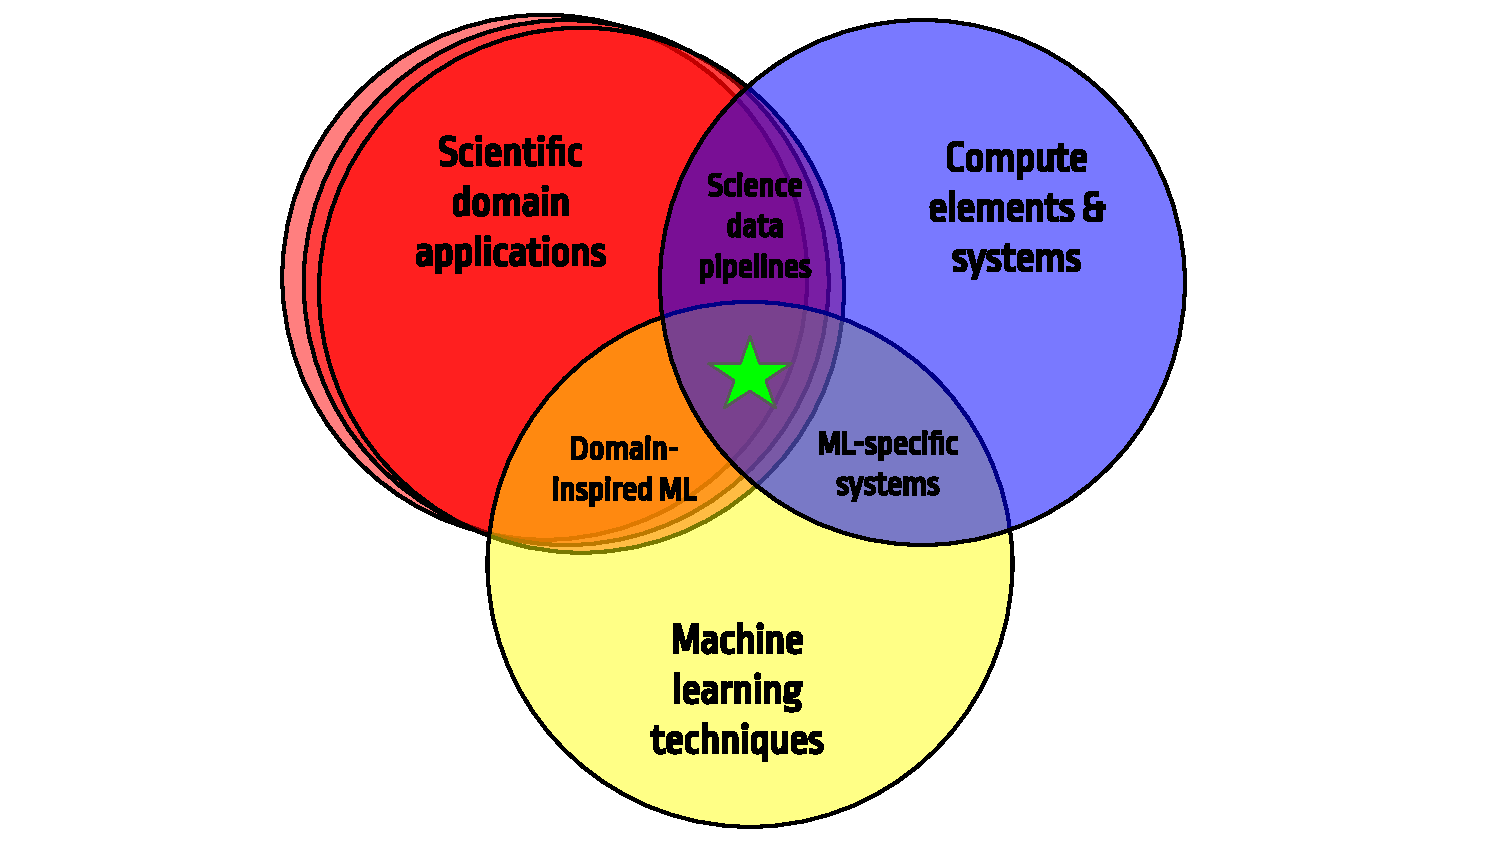
\includegraphics[width=0.6\textwidth]{figures/fastmlintro.pdf}
    \caption{The concept behind this review paper is to find the confluence of domain-specific challenges, machine learning, and experiment and computer system architectures to accelerate science discovery.}
    \label{fig:intro}
\end{figure}


As ML tools have become more sophisticated, much of the focus has turned to building very large  algorithms that solve complicated problems, such as a language translation, and voice recognition. 
However, in the wake of these developments, a broad range of scientific applications have emerged that can benefit  greatly from the rapid developments underway. 
Furthermore, these applications have diversified as people have to come realize how to adapt their scientific approach so as to take advantage of the benefits originating from the AI revolution. 
%Fast Machine Learning within Science has a broad range of applications. 
This can include the capability of AI to classify events in real time, such as the identification of a collision of particles or a merger of gravitational waves. 
It can also include systems control, such as the response control from feedback mechanisms in plasmas and and particle accelerators. 
The latency, bandwidth, and throughput restrictions and the reasons for such restrictions differ within each system. However, in all cases, accelerating ML is a driver in the design goal. 

Design of low latency algorithms differ from other AI implementations in that we must tailor specific processing hardware to the task at hand increase the overall algorithm performance. 
In particular, certain processor cores have been configured for optimized sparse matrix multiplications. 
Others have been optimized to maximize the total amount of compute. 
Processor design, and the design of algorithms around processors,  often referred to as hardware AI co-design, is the focus of the work in this review. 
For example, in some cases, ultra-low latency inference times are needed to perform scientific measurements. 
One must efficiently design the algorithm to optimally utilize the hardware constraints available while preserving the algorithm performance within desired experimental requirements. This is the essence of hardware AI co-design.

The contents of this review are laid out as follows.  In the Section~\ref{sec:apps}, we will explore a broad range of scientific problems where Fast ML can act as a disruptive technology to the status quo and lead to a significant change in how we process data.  
Domain experts from seemingly different domains are examined.  In Section~\ref{sec:overlaps}, we describe  data representations and experimental platform choices are common to many types of experiments.  
We will connect how Fast ML solutions can be generalized to low latency, highly resource efficient, and domain-specific deep learning inference for many scientific applications. Finally in Section~\ref{sec:technolog_sota}, to achieve this requires optimized hardware-ML co-design from the algorithm design to the system architecture.  
We provide an overview of state-of-the-art techniques to train neural networks optimized for both performance and speed, survey various compute architectures to meet the needs of the experimental design, and outline software solutions which optimize and enable the hardware deployment.    

The goal of this paper is to bring together scientific opportunities, common solutions,
and state-of-the-art technology into one single narrative. We hope this can contribute to accelerate the deployment of potentially transformative ML solutions to a broad range of scientific fields going forward. 


% In this document, we will focus on developments of scientific applications where "Fast Machine Learning" is required. "Fast Machine Learning" constitutes broadly the region where AI algorithms are needed to run at low latency. Low latency processes are processes that require fast reaction times so that specific scientific processes can be observed or systems can be controlled in real time. Low latency AI differs from other AI developments in that there is an explicit focus on attaining AI inference with the smallest possible latency. This work differs from AI design of high throughput systems where the aim is to perform as many as possible  operations over a longer period of time so that the throughput aggregated over time is as large as possible. 

% Fast Machine Learning within Science has a broad range of applications. This can include the use of AI to classify events in real time, such as the identification of collision of particles or a merger of gravitational waves. It can also include  systems control, such as the  response control from feedback mechanisms in plasmas and and particle accelerators. The latency restrictions and the reasons for such restrictions differ within each system. However, in all cases, latency is a driver in the design goal with faster inference times generally being better. 

% AI algorithms designed for low latency differ from other algorithm designs in their need to enable low latency. Design's for low latency first aim to ensure that an algorithm is efficiently designed. Small algorithms are typically much more efficient that large algorithms. Consequently, low latency AI algorithm design focuses on approaches to systematically shrink the size of algorithms while preserving the algorithm performance within a desired constraint. 

% Design of low latency algorithms can also differ from that of other AI implementations in that specific processing hardware can be used to increase the overall algorithm performance. In particular, certain processor cores have been configured for optimized sparse matrix multiplications. Others have been optimized to maximize the total amount of compute. Processor design, and the design of algorithms around processors,  often referred to as hardware AI co-design, is the focus of the work in this review. 

% In the following sections, we will explore a broad range of scientific problems where fast machine learning can act as a disruptive technology and lead to a signficant change in how we process data. In particular, we will show how concepts from fast machine learning can lead to ultra fast deep learning inference. Furthermore, fast machine learning can lead to low power, high performance, deep neural networks. The gains that are being observed when optimized hardware ai co-design is present is substantial, and likely to be transformative to a broad range of fields going forward. 


%How to make a dee
%The origins

%look across the wide range of machine learning architectures and try to understand ho we can make machine learning algorithms run fast. 

%The challenge of fast machine learning falls in 